\documentclass[12pt, a4paper]{memoir} % for a short document
\usepackage[french,english]{babel}

\usepackage [vscale=0.76,includehead]{geometry}                % See geometry.pdf to learn the layout options. There are lots.
%\geometry{a4paper}                   % ... or a4paper or a5paper or ... 
%\geometry{landscape}                % Activate for for rotated page geometry
%\OnehalfSpacing
% \setSingleSpace{1.05}
%\usepackage[parfill]{parskip}    % Activate to begin paragraphs with an empty line rather than an indent


%===================================== packages
\usepackage{lipsum}
\usepackage{graphicx}
\usepackage{amsmath}
\usepackage{fullpage}
\usepackage{mathptmx} % font = times
\usepackage{helvet} % font sf = helvetica
\usepackage[latin1]{inputenc}
\usepackage{relsize}
\usepackage[T1]{fontenc}
\usepackage{tikz}
\usepackage{booktabs}
\usepackage{textcomp}%textquotesingle
\usepackage{multirow}
\usepackage{pgfplots}
\usepackage{url}
\usepackage{footnote}
\usepackage{subcaption}
\usepackage{amsfonts}
\usepackage{listings}
\usepackage{xcolor}
\usepackage{float}
\usepackage{wrapfig}

\definecolor{codegreen}{rgb}{0,0.6,0}
\definecolor{codegray}{rgb}{0.5,0.5,0.5}
\definecolor{codepurple}{rgb}{0.58,0,0.82}
\definecolor{backcolour}{rgb}{0.95,0.95,0.92}

\lstdefinestyle{mystyle}{
    backgroundcolor=\color{backcolour},   
    commentstyle=\color{codegreen},
    keywordstyle=\color{magenta},
    numberstyle=\tiny\color{codegray},
    stringstyle=\color{codepurple},
    basicstyle=\ttfamily\footnotesize,
    breakatwhitespace=false,         
    breaklines=true,                 
    captionpos=b,                    
    keepspaces=true,                 
    numbers=left,                    
    numbersep=5pt,                  
    showspaces=false,                
    showstringspaces=false,
    showtabs=false,                  
    tabsize=4
}

\lstset{style=mystyle}

\newcommand{\IFa}{\uparrow\mathrm{IF}}
\newcommand{\IFr}{\downarrow\mathrm{IF}}
\newcommand{\IDa}{\uparrow\mathrm{ID}}
\newcommand{\IDr}{\downarrow\mathrm{ID}}
\newcommand{\FUa}{\uparrow\mathrm{FU}}
\newcommand{\FUr}{\downarrow\mathrm{FU}}
\newcommand{\COM}{\mathrm{COM}}

% \newcommand{\TODO}[1]{\colorbox{red!30}{TODO: \textbf{#1}}}
\newcommand{\TODO}[1]{}

\usepackage[most]{tcolorbox}
\newcounter{example}
\newtcolorbox{examplebox}[2][]{
    colback=gray!10,
    colframe=gray!80,
    boxrule=0.5pt,
    arc=3pt,
    left=6pt,
    right=6pt,
    top=4pt,
    bottom=4pt,
    fonttitle=\bfseries,
    title={Example~#2:~#1}
}
\newenvironment{example}[1][]{
    \refstepcounter{example}
    \begin{examplebox}[#1]{\theexample}
}{
    \end{examplebox}
}

\newcounter{assumption}
\newtcolorbox{assumptionbox}[2][]{
    colback=blue!5,
    colframe=blue!40,
    boxrule=0.5pt,
    arc=3pt,
    left=6pt,
    right=6pt,
    top=4pt,
    bottom=4pt,
    fonttitle=\bfseries,
    title={Assumption~#2:~#1}
}
\newenvironment{assumption}[1][]{
    \refstepcounter{assumption}
    \begin{assumptionbox}[#1]{\theassumption}
}{
    \end{assumptionbox}
}


\begin{document}
\chapter*{Towards a New Causality Definition}

This is a draft, where I describe my ideas regarding the notion of causality and how it should be modified. Here I include the things I had no time to include in the internship report which was prepared for internship defense. Please look into the report for more details.

\TODO{add abstract}

\textit{Made by Andrei Ilin on \today.}

\section{The Limitations of Binder's Definition}

As shown in the report, the definition of Binder et al. is susceptible to the \textit{gap problem}. Two events $e_1$ and $e_2$ can be connected with causality links only if they are connected via ETDG link and there is no event $e_3$ s.t. $e_3 \rightarrow e_2 \in ETDG$ and $e_3.t > e_1.t$. 

But why do we argue that $e_1$ and $e_2$ should be causally connected? In the example the pair of traces $\alpha$ and $\beta$ exhibits only one variation, which is in latency of instruction $A$. Thus, all the events $e$ s.t. $e^\alpha.t \ne e^\beta.t$ are caused by this variation.

Our goal is to define a new notion of causality that would be able to capture all affected events. Let us start with formulating the expected properties of hypothetical causality definition. Consider two traces $\alpha$ and $\beta$ where $\alpha$ has a single variation compared to $\beta$. We explore a causality links in $\alpha$.

The definition of causality is expected to have the following properties:
\begin{enumerate}
    \item \textbf{Reachability} --- Any event whose timestamp is different between traces $\alpha$ and $\beta$ must be causally linked to the variation.
    \item \textbf{Correctness} --- If an event is reachable via causal links, it has different timestamps between $\alpha$ and $\beta$.
    \item \textbf{Forwardness} --- Given a causality link $e_1 \rightarrow e_2$, $e_1$ happens earlier than $e_2$ in trace $\alpha$.
\end{enumerate}


\section{Introducing Resolution Procedure}

\subsection{Event-Based Approach}

\TODO{input: known latencies}

Here we do not take into account branch prediction. Consider single-issue processor.

In our method we focus solely on events in the execution traces. We establish a set of rules which can uniquely define the scheduling inside the processor pipeline.

First, each type of event we define the constraints for timestamp.
\begin{enumerate}
    \item $\IFa$ --- not earlier than $\IFr$ of previous instruction.
    \item $\IFr$ --- at least 1 cycle must pass since $\IFa$ of the same instruction.
    \item $\IDa$ --- not earlier than $\IDr$ of previous instruction, not earlier than $\IFr$ of the same instruction.
    \item $\IDr$ --- at least 1 cycle must pass since $\IDa$ of the same instruction.
    \item $\FUa$ --- not earlier than $\IDr$ of the same instruction. Cannot be placed between $\FUa$ and $\FUr$ of the same FU by other instruction (exception: can be placed on the same cycle as $\FUa$ of later instruction. The exception depends on scheduling policy). Not earlier than $\FUr$ of instructions from dependencies.
    \item $\FUr$ --- at least \textit{latency} cycles must pass since $\FUa$ of the same instruction.
    \item $COM$ --- not earlier than $\FUr$ of the same instruction. At least 1 cycle must pass since $COM$ of previous instruction.
\end{enumerate}

Second, to uniquely determine the position of event, there should not exist the earlier position where the event can be placed. In other words, each event is scheduled as soon as it is possible by the constraints.

If the rules hold true for an event $e$, we call $e$ \textit{stable} and \textit{unstable} otherwise. The \textit{stable} set of events is a set where every event is stable.

\textbf{Proposition 1:} For any given input there is only one stable set of events, which corresponds to the set of events derived from execution on the model of the processor.

\subsection{Step-by-Step Resolution}

The idea is that each the rules correspond to the possible dependencies between events (ETDG arcs from Bidner's definition).

Our notion of causality relies on information of both execution traces. The intuition behind our approach is following: if an event $e_2$ changed its timestamp from trace $\beta$ to trace $\alpha$, its movement is either because of variation or the movement of some other event $e_1$. In the second case, the causal link $e_1 \rightarrow e_2$ must be established.

Given a set stable set of events $E$ that represents the execution trace, we introduce a variation by changing the latency of one of the instructions. This creates a new set of constraints $C$. Because of the proposition 1, $E$ is not stable with respect to $C$, therefore we have a subset of unstable events $U_1 \subset E$. We resolve $E$ by moving all the events form $U$ to the stable position (each to the earliest position where the set of rules hold). However, this creates a set of new unstable events $U_2 \subset E$. We resolve them and repeat the procedure until $U_n = \emptyset$.

\textbf{Proposition 2:}
The resolution procedure always terminates.

\textbf{Proposition 3:}
The procedure resolves in trace with corresponding to the execution trace of modified input.

Proposition 3 directly follows from propositions 1 and 2.

We illustrate how the resolution procedure works on an example. Consider a following input:

\begin{tabular}{r|ccc}
 & Res & Dep. & Lat. \\ \hline
\textit{A:} & FU1 &  & $4|1$ \\
\textit{B:} & FU2 & $\{A\}$ & $4$ \\
\textit{C:} & FU2 &  & $4$ \\
\textit{D:} & FU1 & $\{C\}$ & $4$ \\
\end{tabular}

It creates a pair of execution traces $\alpha$ and $\beta$ with latency of $A$ being 4 and 1 in $\alpha$ and $\beta$ respectively. Figure \ref{fig:causality-resolution-example} shows the resolution procedure for this input. We start from trace $\beta$, from which we get $\beta_1$ by changing the latency of $A$. Then, on each step unstable events are identified (shown in red boxes) and moved to new positions (shown as green boxes). Note that here we synchronzie the movement of $\FUr$ to the movement of corresponding $\FUa$: this is done for simplicity of visualization. Formally, the described procedure must move $\FUa$ first, and only in the next resolution step the $\FUr$ will be moved. The example illustrates how through a number of resolution step trace $\beta$ turns into $\alpha$.


\begin{figure}[H]
    \centering
    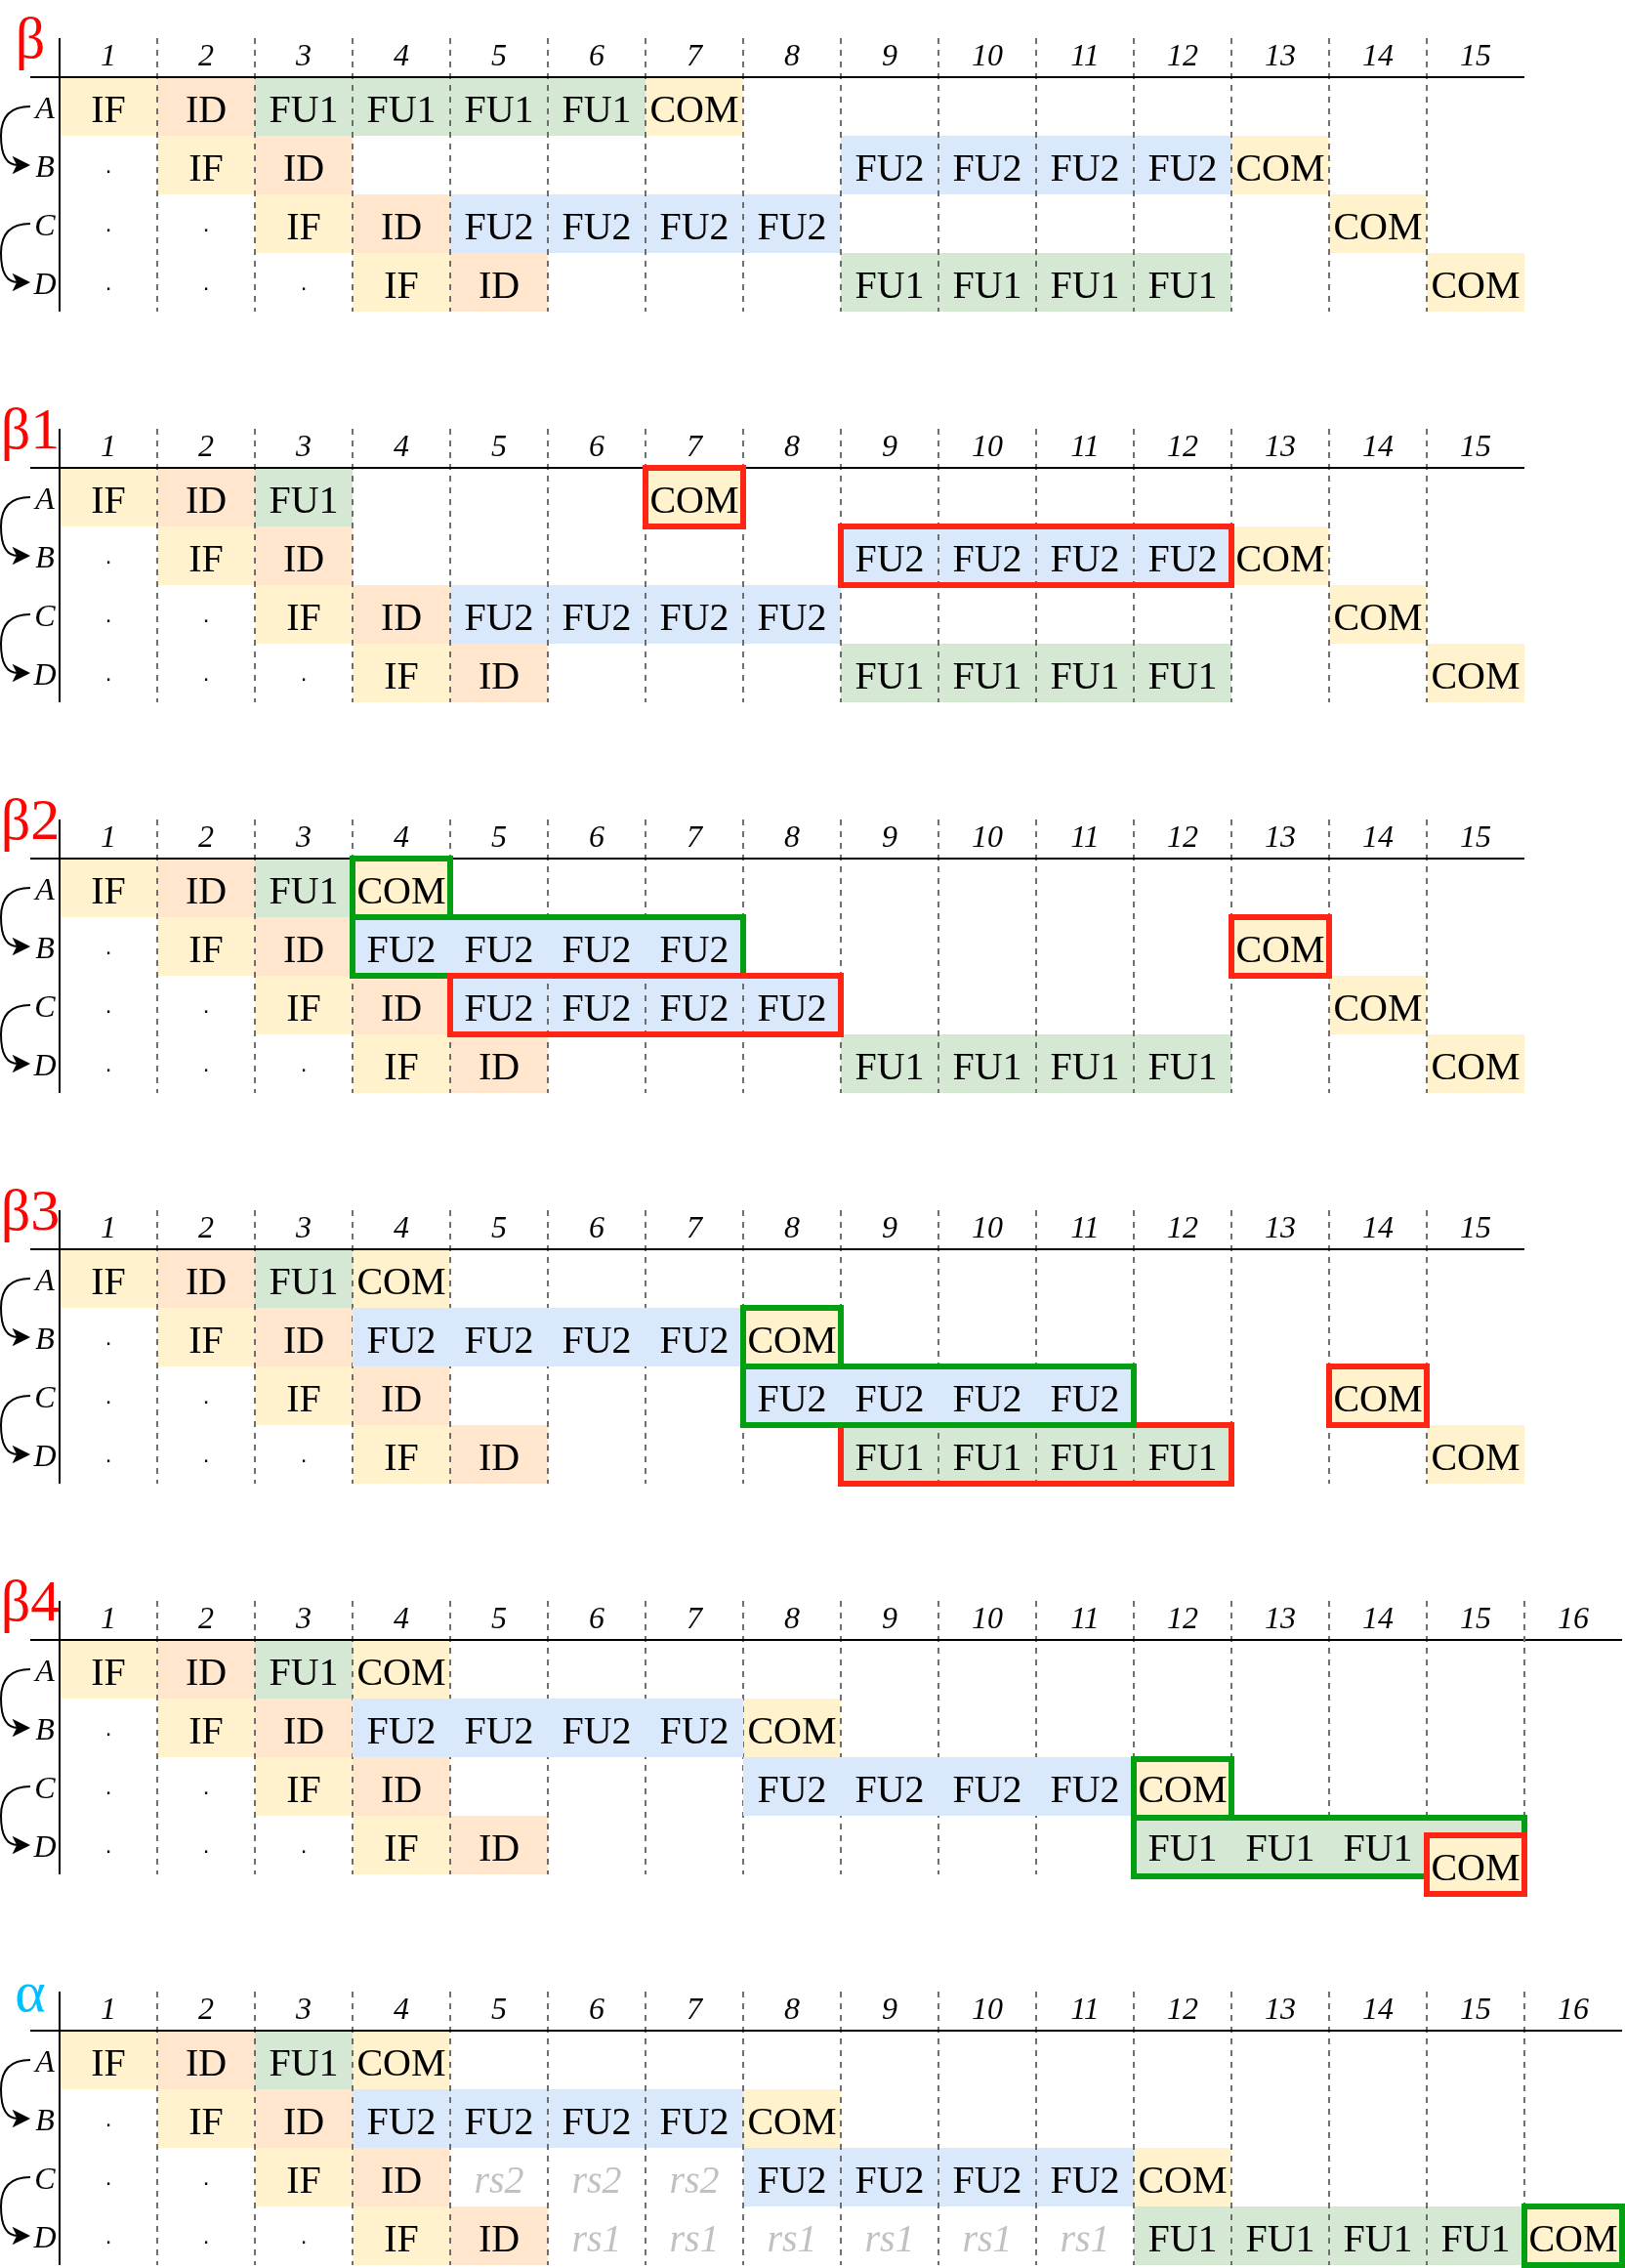
\includegraphics[width=0.7\textwidth]{pics/resolution-steps-example.png}
    \caption{An example illustrating the step-by-step resolution procedure}
    \label{fig:causality-resolution-example}
\end{figure}

\subsection{Deriving Causality from Resolution Procedure}

The resolution procedure gives us some information about the order of which the events influence each other. We try to define the causality from the resolution procedure as follows:

Consider 3 event sets $E_1, E_2, E_3$ where the events are different only by timestamps. They represent a part of the resolution procedure ($E_1 \xrightarrow{U_1} E_2 \xrightarrow{U_2} E_3$), where $U_1$ is a set of events moved in step $E_1 \rightarrow E_2$, $U_2$ - a set of events moved from $E_2 \rightarrow E_3$. We establish the causality relations between events from $U_1$ to events from $U_2$. To determine which events are responsible for $u \in U_2$ to move, we find the smallest subset $U_1' \subseteq U_1$ s.t. $E_1 \xrightarrow{U_1'} E_2' \xrightarrow{U_2'} E_3'$ and $u \in U_2'$. In other words, we search for which events are enough to move in the first step to observe $u$ be moved in the next. Thus, each event may have several incoming multiedges (there can be multiple subsets found). Subsets are disjointed.

\textbf{Filtering}

When applying the procedure some event may be moved several times, so we keep only the arcs corresponding to the last movement of the event.

Figure \ref{fig:successful-res} shows the connections restored from example above.

\begin{figure}[H]
    \centering
    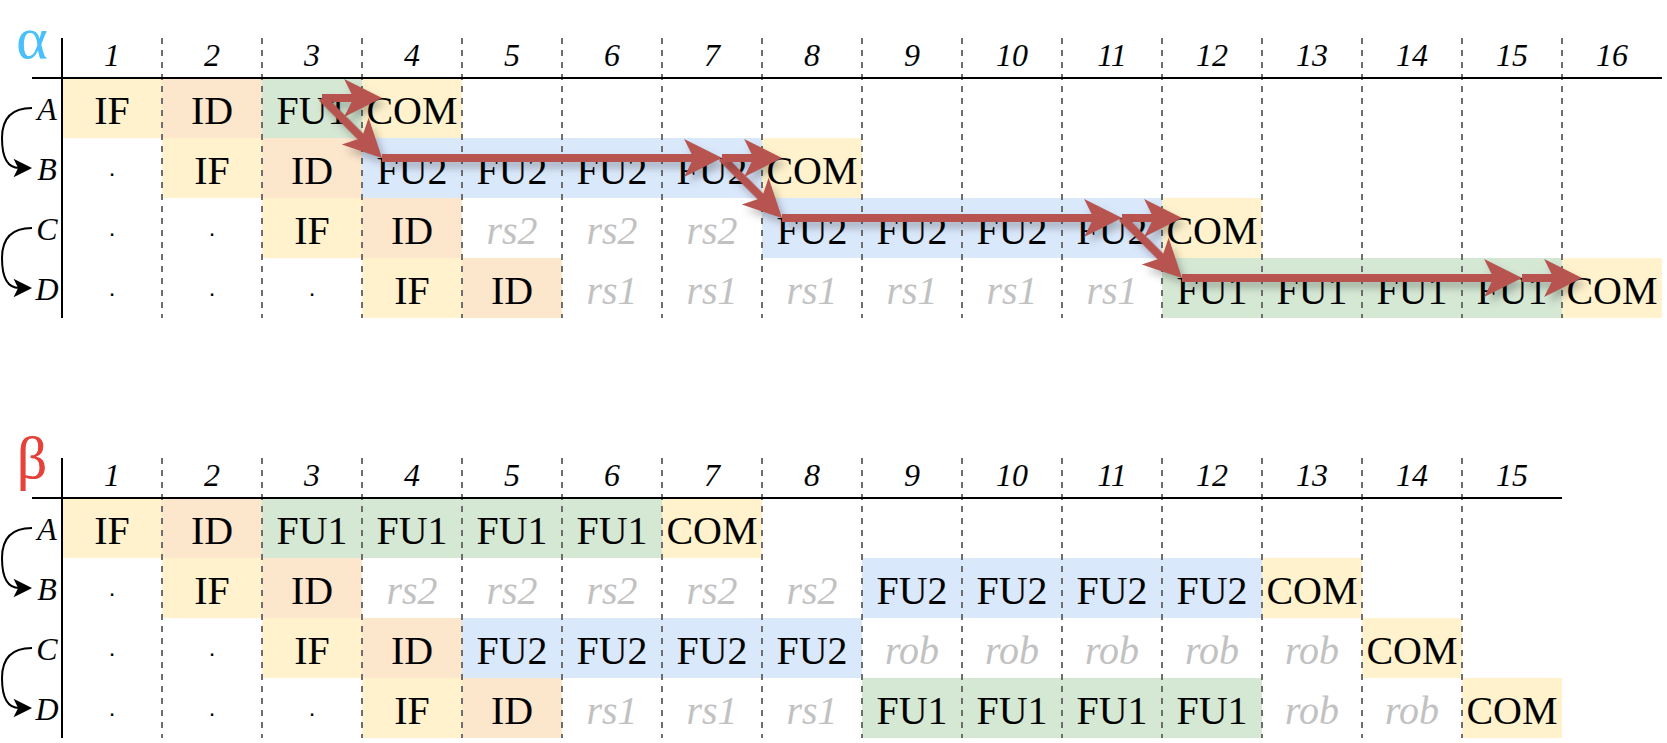
\includegraphics[width=0.7\textwidth]{pics/successful-res.png}
    \caption{Graph restored form resolution procedure shown in figure \ref{fig:causality-resolution-example}}
    \label{fig:successful-res}
\end{figure}

Figure \ref{fig:multiedge} shows an example of multiedge: since execution of $D$ is restricted by $B$ and $C$, both $B$ and $C$ must move to allow $D$ to move.

\begin{figure}[H]
    \centering
    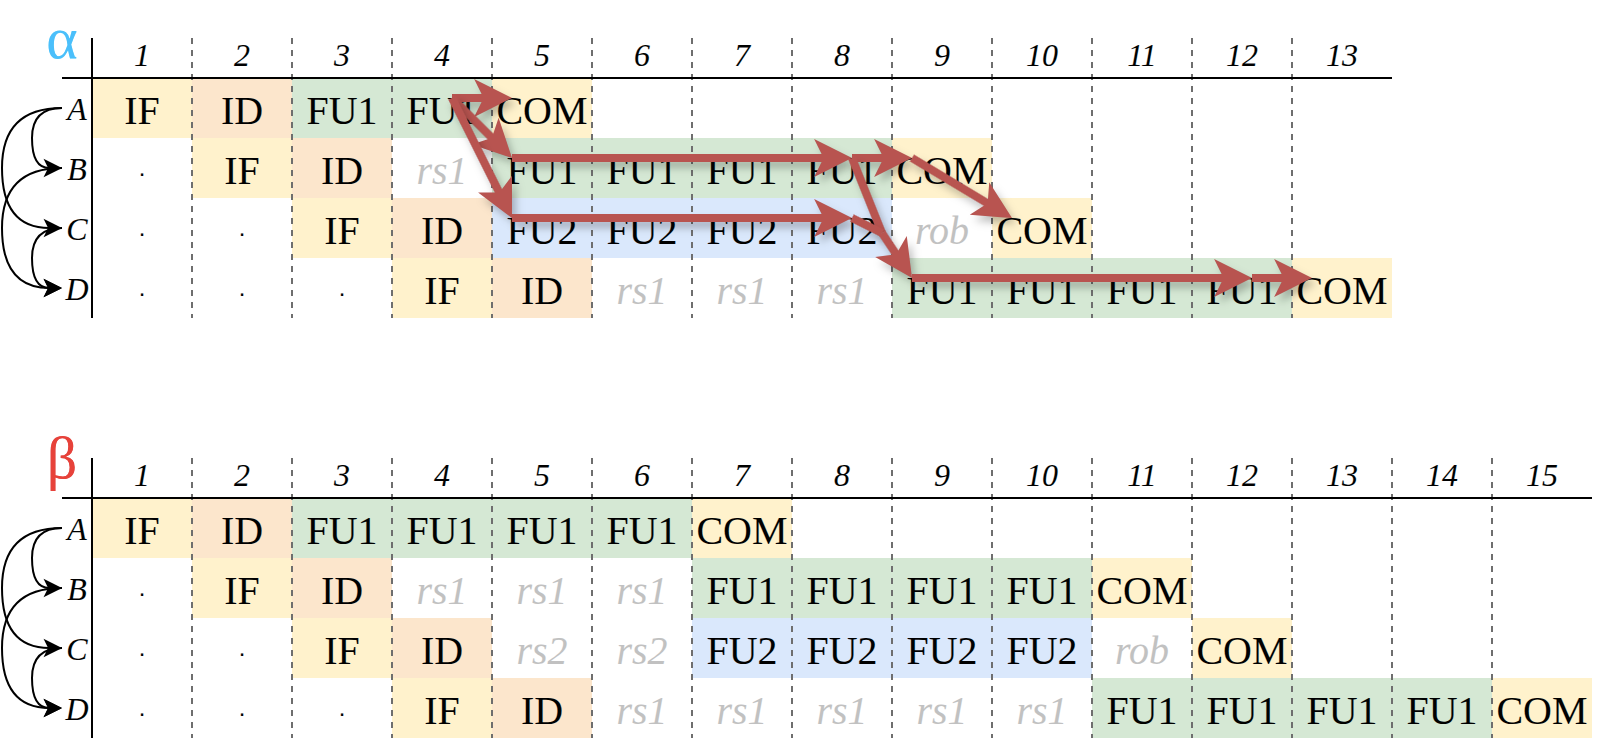
\includegraphics[width=0.7\textwidth]{pics/multiedge.png}
    \caption{Multiedge example}
    \label{fig:multiedge}
\end{figure}

\textbf{Filtering problem}

Example in figure \ref{fig:filter-problem} is similar to one from figure \ref{fig:multiedge}. However, here instruction $C$ is split into two: $C$ and $D$. Normally, we would expect ot see a multiedge $(B,D) \rightarrow E$ here. However, due to the filtering we detect the edge $D \rightarrow E$ later than $B \rightarrow E$ and the priority is given to the last discovered.

So the filter should be implemnted differently.

\begin{figure}[H]
    \centering
    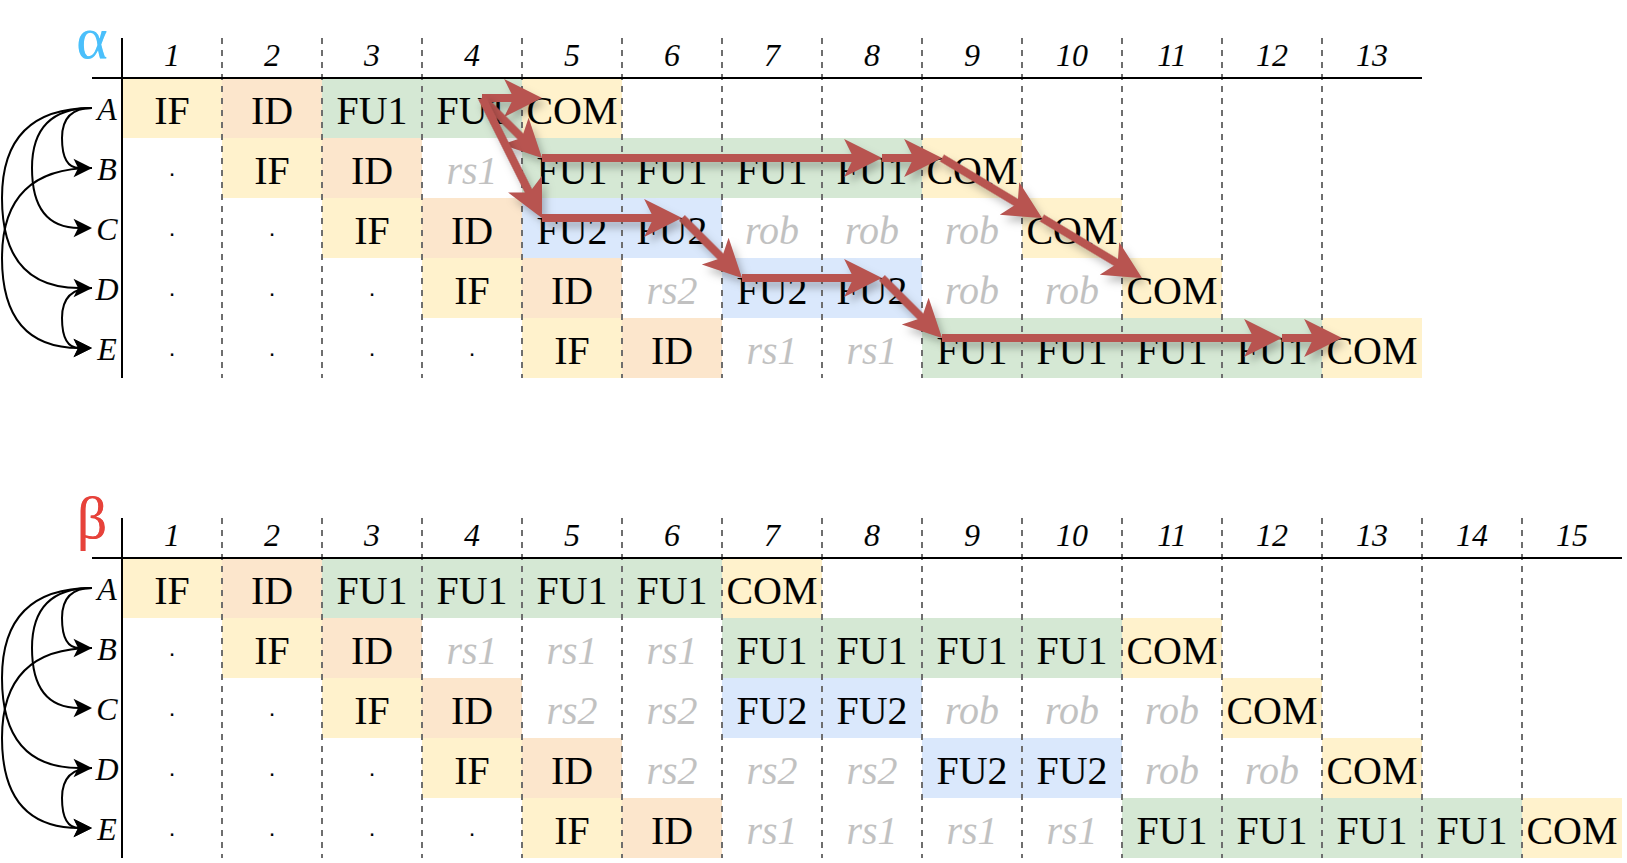
\includegraphics[width=0.7\textwidth]{pics/filter-problem.png}
    \caption{Missing edge}
    \label{fig:filter-problem}
\end{figure}


\TODO{moving from alpha to beta}

\end{document}